\documentclass[11pt, a4paper]{report}
\usepackage[utf8]{inputenc}
\usepackage{float}
\usepackage{array}
\usepackage{amsmath}
\usepackage{amssymb}
\usepackage{amsfonts}
\usepackage{latexsym}
\usepackage{graphicx}
\usepackage{tabularx}
\usepackage{ltxtable}
\usepackage{longtable}
\usepackage{color, colortbl}
\usepackage{caption}%\usepackage{subcaption}
\usepackage{ifpdf}
\usepackage[hidelinks]{hyperref}
\usepackage{url}
\usepackage{xtab}
\usepackage[hmargin=3cm,vmargin=3cm]{geometry}
\usepackage[norsk, english]{babel}
\usepackage[parfill]{parskip}
\usepackage{pdfpages}
\usepackage{listings}
\usepackage{subfigure}
\usepackage{xcolor,colortbl}

% Begin chapter numbering
\usepackage[T1]{fontenc}
\usepackage{titlesec, blindtext, color}

\definecolor{gray75}{gray}{0.75}
\newcommand{\hsp}{\hspace{20pt}}
\titleformat{\chapter}[hang]{\Huge\bfseries}{\thechapter\hsp\textcolor{gray75}{|}\hsp}{0pt}{\Huge\bfseries}
% End chapter numbering

% Add numbering to subsubsection
\setcounter{secnumdepth}{3}
\setcounter{tocdepth}{3}

\definecolor{Gray}{gray}{0.9}

% Header packages
\usepackage{fancyhdr}
\pagestyle{fancy}
\rhead{Chapter: \thechapter}

% Custom
%\newcommand{\newCommandName}{text to insert} % Defines a variable in LaTeX
\newcommand{\comment}[1]{} \comment{This is a block comment wrapped in curly brackets}
%\renewcommand{\thefootnote}{\roman{footnote}}

\begin{document}
%\pagecolor{yellow!30} % Uncomment for debugging floats
\pagenumbering{gobble}


\begin{titlepage}
\begin{center}
\vspace*{1in}
{\LARGE Eksperter i Team}
\par
\vspace{1cm}


\begin{figure}[ht!]
\centering
%
\includegraphics[width=25mm]{images/logo.png}
%\caption{A simple caption}
\label{overflow}
\end{figure}


{\LARGE Stereo}
\par
\vspace{0.6in}
{\LARGE Project report}
\par
\vspace{0.2in}
{\Large Group 1}
\par
\vfill
\par
\vspace{0.5in}
Our names\\ \ldots here\\
\par
\vspace{0.4cm}
\today
\end{center}
\end{titlepage}

%\newpage
%
%\input{section/abstract}

\tableofcontents
\newpage
\pagenumbering{arabic}

%%%
% Put new includes here
%%%

%\chapter{Introduksjon}
\section{Gruppen} 
\subsection{Emil Bjørlykhaug}
Går undervannsteknologi, 2-årig master. Har tidligere gått Automasjon ved Hials.
Som folk flest hadde jeg hørt en del snakk om EiT på forehand, noe positivt, noe negativt. 
Jeg hadde ikke noen store forventninger ang. selve prosjektet vi skulle gjennomføre,
 men hadde en del forventninger til det å jobbe i gruppe, og å lære hvordan gruppedynamikk 
fungerer sett fra både et teoretisk og praktisk perspektiv. Jeg har tidligere selv jobbet 
en del i grupper, men oftest har medlemmene av desse gruppene vært folk jeg har kjent 
fra før. I et tilfelle når jeg studerte på Hials hadde foreleser ansvaret med å dele opp gruppe, 
så jeg havnet på en gruppe med bare ukjente personer. Jeg følte dette er en god måte å 
utfordre folk sosialt, og følte jeg i løpet av semesteret ble utrolig godt kjent med de jeg 
måtte jobbe sammen med.
Jeg er ikke av typen som roper høgest i diskusjoner, og kan ofte bli litt passiv i 
gruppesammenhenger om jeg ikke føler jeg har noe å stille med, men håper 
EiT kan gjøre meg til et bedre gruppemedlem. Jeg er positivt innstilt til faget 
og håper på høgt læringsutbytte.

\subsection{David Hovind} Jeg har ikke hørt så mye om EiT fra før så jeg vet ikke helt hva det går ut på. 
Jeg har derfor et åpent sinn til faget og ser på det som en positiv utfordring. 
Som regel så foretrekker jeg ikke gruppearbeid fordi man blir avhengig av alle andre i gruppen og de blir avhengige av deg. 
Av den grunn så liker jeg best å jobbe selvstendig, siden det finnes mange forskjellige typer mennesker og man vet aldri 
hvilke typer mennesker man havner på gruppe med. Jeg forventer å bli bedre til å kjenne meg selv og få litt innsikt i 
hvordan det er å reflektere over gruppearbeidet.

\subsection{Kristoffer Løvall}
Jeg fikk høre litt forskjellig om Eksperter i Team før dette semesteret, men har 
prøvd å holde de negative holdningene til faget ute. Jeg starter semesteret 
derfor semesteret med en positiv innstilling, spesielt siden landsbyens tema 
virker veldig interessant og spennende. Jeg forventer at det blir lærerikt å 
jobbe på tvers av fagfelt og interesser, og at tverrfagligheten bidrar til å 
designe et godt produkt. På grunn av tidligere gruppearbeid i forhåndsbestemte 
grupper med ukjente personer har jeg ikke store forventninger til det sosiale, 
noe som på sitt vis kan være positivt ettersom det da ikke er mye som skal til 
for at dette går over forventning. Jeg har også jobbet relativt mye i grupper 
gjennom porsjekter både på NTNU og Høgskolen i Bergen, der jeg ofte har endt opp 
med å ta ansvar og fungere som en gruppeleder. Jeg vet også at jeg kan bli noe 
kontrollerede når jeg blir veldig engasjert og brenner for noe.  Målet mitt for 
Eksperter i Team er å "prøve noe nytt" og være litt mer tilbakeholden på denne 
fronten, prøve å jobbe på linje med alle andre uten å "ta over" for noen og 
kontrollere alle detaljer. Jeg vil bli enklere å jobbe i team med og lære meg 
selv å godta andres løsninger og akseptere disse som de beste løsningene, selv om 
min opprinnelige tanke var noe helt annet. Når det gjelder det faglige håper jeg 
alle har høye forventninger både når det gjelder engasjement for å ende opp med 
gode løsninger, samt det å få en god karakter i faget.
\section{Hardware}

Hardware (HW) omfatter systemet fra sensor til nettverksprotokollen som blir brukt i
bilsystemet. Hvilken HW
som trengs er da avhengig av noen faktorer:
\begin{itemize}
\item Tilgjengelige sensorer
\item Nettverksdata format
\item Nødvendig dataprosessering
\item Utfordringer ved signaloverføring
\item Bruk av nettverksprotokoll
\end{itemize}

Denne seksjonen vil gå nærmere inn på faktorene som er med på å definere og begrense HW design. I tillegg
studeres krav ulike sensorteknologier stiller til HW. Til slutt sammenlignes ulike HW design.

%hvilke sensorer som er tilgjengelige, hvilke data
%man får fra de ulike sensorene, hvilken dataprosessering som er nødvendig og
%utfordringer i forhold til signaloverføring og
%hvilken nettverksprotokoll som brukes. \\

\subsection{Definerende og begrensende faktorer}

En definerenede faktor for HW er måleteknikk. Det er da særlig krets
mellom eventuelt mikrokontroller (MCU) og sensor som vil variere. Ulike måleteknikker studeres
i seksjon \ref{subsec:sensorteknologier}. Måleteknikken setter også en begrensing på hva som er
mulig å måle og dermed hvilke tjenester systemet kan tilby. \\

I bilindustrien er CAN den rådende nettverksprotokollen \cite{canbus}. Man
kan argumentere for at man på grunnlag av dette burde integrere nye systemer på
det eksisterende nettverket. Uansett hvilket nettverk det skal kommuniseres over
vil det stille krav til HW. En ny enhet bør ha riktig nettverksgrensesnitt
og må kunne kommunisere på riktig protokoll. \\

\subsection{Sensorteknologier}
\label{subsec:sensorteknologier}

Det er flere fysiske prinsipper som kan måles for å detektere en løs hjulmutter.
Det er derfor viktig å undersøke hvilke sensorteknologier som er tilgjengelig og
hvilke fordeler disse drar med seg. \\

Tre ulike fysiske prinsipper som kan brukes er strekk, trykk og vibrasjon. \\

\subsubsection{Vibrasjonsmåling}

Vibrasjonsmåling kan bli gjort med teknologier som et akselerometer eller ved
pizoelektriske mikrofoner. Slike sensorer vil kunne gi et signal som inneholder
ulike frekvenstyper som kan analyseres. Slik kan man gjenkjenne mønstre i
frekvensbåndet som indikerer eksempevis en løs mutter. For å analysere dette signalet må det
samples med en Analog-til-Digital Converter (ADC). Dersom signalet er svakt må det også forsterkes gjennom en
forsterker krets. 

For å hente ut informasjon av signalet må en algoritme undersøke
frekvensoppbyggingen av signalet. Dette kan bli gjort i HW med en Digital Signal Processor (DSP), men kan
også gjøres i software (SW) ved at det sendes en signalprøve fra HW til kontrolsystemet. Å
bruke en DSP kompliserer HW og effektforbruk og kost øker. Det krever også at algoritmen på DSP'en 
er lastet inn før den brukes og kan ikke endres uten at den omprogrammeres. Analyseres signalene i HW kan vil
det kunne sendes korte datapakker på Can bussen og sampling av signalet vil kunne gjøres kontinuerlig. Dette er
positivt med tanke på å ikke overbelaste CAN bussen som brukes av mange andre enheter i bilen. 

Analyserer man signalet i SW blir det lettere å oppdatere algoritmen etter installasjon av HW
samt at det kan benyttes artificial intellegence (AI) til å justere algoritmen bassert på målinger underveis. 
Dette forenkler HW litt ved at man ikke trenger en DSP krets, men HW blir nødt å sende større pakker over CAN
bussen. Dette kan potensielt bruke opp båndbredden til CAN bussen dersom store pakker med data sendes ofte. 
Det er vitkig å komme frem til en akseptabel størrelse på samplingsdataen som skal sendes samt frekvensen på
sendingen. Dette avgjøres i storgrad av den eksisterende trafikken på CAN bussen.

%Tanken er å ha sensoren på akslingen mellom to hjul. For å skille mellom hvilket
%hjul som har løse muttere, så kan det være en løsning å bruke en sensor ved vært
%hjul. Da er to mulig algoritmer å måle amplitudeforskjell eller
%tidsforsinkelse. Dette burde være mulig å få til med en MCU, men kan være det
%blir nødvendig med en DSP for raskere prosessering av signalene. \\
%
%MCUen sender pakkene med en ID slik at man kan skille mellom ulike akslinger. \\

\subsubsection{Strekklapper/Trykklapper}

Tanken er å legge strekklapper inni eller på utsiden av boltene eller
trykklapper mellom bolt og nav. Strekklappene
må/kan/bør legges i en krets (Wheatstone feks) for å kunne gi ut et målbart
spenningsnivå. For å oppnå et målbart spenningsnivå må man mest sannsynlig
forsterke signalet gjennom en In Amp. Denne analoge målingen krever mye lavere sampling end ved
vibrasjonsmålinger da det trengs kortere signalprøver.
Man kan få problemer med at signalet fra strekklappen må gjennom en slepering.
Dette kan by på utfordringer med tanke på implementasjon og støy.
Man må også ha en sensor per bolt. Dette fører til mer HW. En måte å redusere
mengden HW på kan være å MUX'e signalene fra hver sensor til MCU. Det er mulig å lage
en krets hvor man benytter seg av tidskonstanten i en RC-krets (dette må du
undersøke litt). Overføring av
signaler fra nav til aksling kan også skje ved induksjon (dette må du undersøke
litt mer). For å koble til flere
enheter på et CAN bus så kan man benytte seg av J1939 som fordelere ID på
nettverket (dette må du undersøke litt mer). \\

\begin{figure}[H]
\subfigure[]{
	
\includegraphics[width=0.4 \textwidth]{images/Straingage_vector.png}
	\label{fig:Strekklapp_vector}
	}
\hfill
\subfigure[]{
	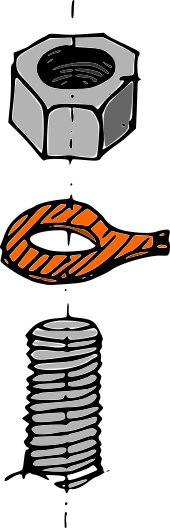
\includegraphics[width=0.2 \textwidth]{images/trykklapp_vector.png}
	\label{fig:Trykklapp_vector}
	}
\caption{\protect{\ref{fig:Strekklapp_vector}} Strekklapp i bolt (orange), \protect{\ref{fig:Trykklapp_vector}} Trykklapp (orange) mellom bolt og mutter.}
\end{figure}

\subsection{Utfordringer}

Problemet med å måle vibrasjoner er at en sampleprøve av et signal innenfor et gitt tidsrom kan bli veldig stor. Som
et resultat at de store sampleprøvene kan det oppstå båndbreddeproblemer på CAN-bussen. Grunnen til dette
er at samplingsfrekvensen man sampler signalet med må være
minst dobbelt så høy som frekvensen av signalet, if ølge Nyquist–Shannon sampling theorem \cite{nyquist}. Høyere
samplingsrate gir bedre signalrepresentasjon, og en god
representasjon av signalet kan være viktig for en eventuell analysealgoritme.

Dersom analysealgoritmen kjøres på en DSP slipper CAN-bussen og overbelastes av store datamengder.
Algoritmen ligger ikke da i det sentrale systemet og det kan bli vanskeligere å forbedre algoritmen ved hjelp av AI.


%%%
% End includes
%%%

%\newpage
%\addcontentsline{toc}{chapter}{List of Tables}
%\listoftables
%\addcontentsline{toc}{chapter}{List of Figures}
%\listoffigures
%\addcontentsline{toc}{chapter}{Bibliography}
%\bibliographystyle{plain}
%\input{section/bibliography}

%\newpage
%\addcontentsline{toc}{chapter}{Appendixes} % This line may break your compilation, and may require recompiation. Not to worry though.
%\appendix
%\input{section/appendix-someAppendix}


\end{document}
